% Provenance (never printed): cycle 4 SVT/physique, "La planete Terre,
% l'environnement": the atmosphere, its structure and its layers, pressure
% and altitude, the ozone layer; see sources/book1/PROVENANCE.md. Book 1,
% grade 8, chapter 1.
% Vocabulary guard: owns the layers of the atmosphere (troposphere,
% tropopause, stratosphere, mesosphere, thermosphere), the environmental
% lapse rate and the ozone layer. Air pressure and the barometer are the
% physics books' (recalled), the composition of air and ozone the molecule
% the chemistry books'; "convection cell" is g8.2's and is not used here;
% adiabatic cooling is Book 2's.
\chapter{L'atmosphère}\label{ch:g8:the-atmosphere}

Dans une station \omterm{def:g1:watching-the-weather:weather}{météorologique}, juste avant l'heure convenue, une
météorologue sort sur la pelouse en tenant un ballon gonflé à l'hydrogène
ou à l'hélium, d'environ \qty{1.5}{m} de diamètre. Au-dessous, au bout
d'une longue ficelle, pendent un petit parachute orange et un boîtier
d'instruments de 60 à 80~grammes~: une \emph{radiosonde}. Elle lâche le
ballon. Le ballon monte d'environ \qty{300}{m} chaque minute, et chaque
seconde la radiosonde transmet par radio la pression, la température,
l'humidité et sa position. En montant, le ballon gonfle, jusqu'à atteindre
6 à \qty{8}{m} de diamètre et éclater, souvent à plus de \qty{30}{km}
d'\omterm{def:g4:world-physical-map:altitude}{altitude}, deux heures après le lâcher. Aux mêmes heures, chaque jour, la
même scène se déroule dans plus de 800~stations à travers le monde.
% ledger: nws:radiosonde

\begin{omfigure}
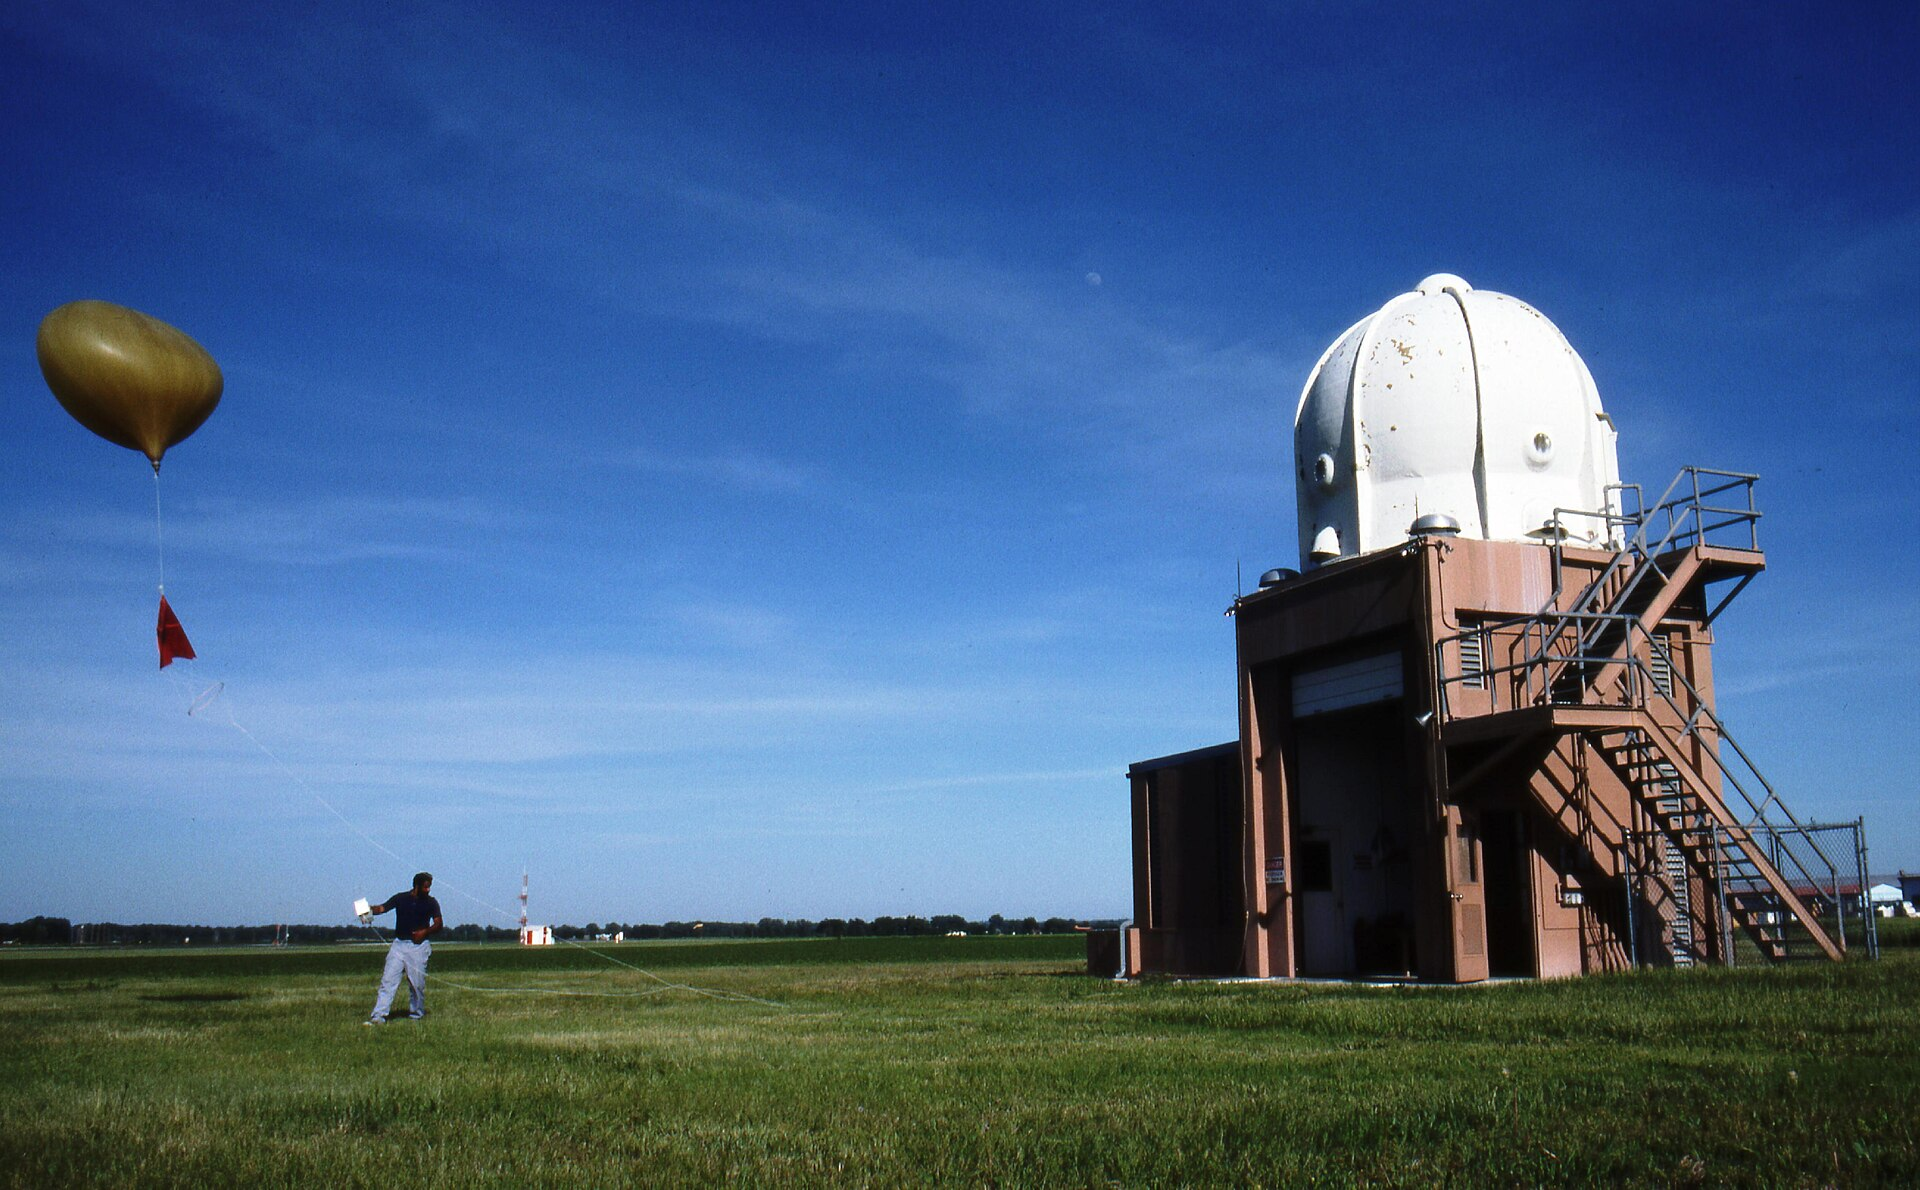
\includegraphics[width=0.78\linewidth]{images/book1/g8-radiosonde-launch.jpg}

{\small Lâcher d'un ballon-sonde à Topeka, au Kansas (États-Unis)~: le
parachute (rouge) et la radiosonde pendent sous le ballon. Photographie de
Stephen Corfidi, NOAA/National Weather Service (domaine public, via
Wikimedia Commons).}
% ledger: commons:radiosonde-launch
\label{fig:g8:the-atmosphere:launch}
\end{omfigure}

Pourquoi le ballon gonfle-t-il en montant~? Que mesure la radiosonde
pendant sa montée, et pourquoi la température ne baisse-t-elle pas
simplement de plus en plus~? Où l'air s'arrête-t-il~?

\begin{recall}
L'\emph{atmosphère} est la couche d'air qui entoure la Terre. L'air
appuie sur tout ce qu'il touche~: c'est la \emph{pression atmosphérique},
que l'on mesure avec un baromètre (les livres de physique). Les services
\omterm{def:g1:watching-the-weather:weather}{météorologiques} la donnent en hectopascals (hPa)~; au \omterm{def:g4:world-physical-map:altitude}{niveau de la mer},
elle vaut environ \qty{1013}{hPa}. L'air sec est fait d'environ 78~\%
d'azote et 21~\% d'oxygène, avec un peu d'argon, de dioxyde de carbone et
d'autres gaz (les livres de chimie). Les \omterm{def:g4:clouds-rain-snow:cloud}{nuages} sont faits de minuscules
gouttelettes d'eau ou de cristaux de glace (\cref{ch:g4:clouds-rain-snow}).
\end{recall}
% ledger: air:N2, air:O2, ussa76:sea-level

\section{Une mince enveloppe}

Vue depuis la Station spatiale internationale, l'atmosphère est une mince
ligne lumineuse le long du bord de la Terre. La plus grande partie de
l'air, et presque tous les \omterm{def:g4:clouds-rain-snow:cloud}{nuages}, se trouvent dans ses quelques
kilomètres les plus bas.
% ledger: commons:iss-sunset

\begin{omfigure}
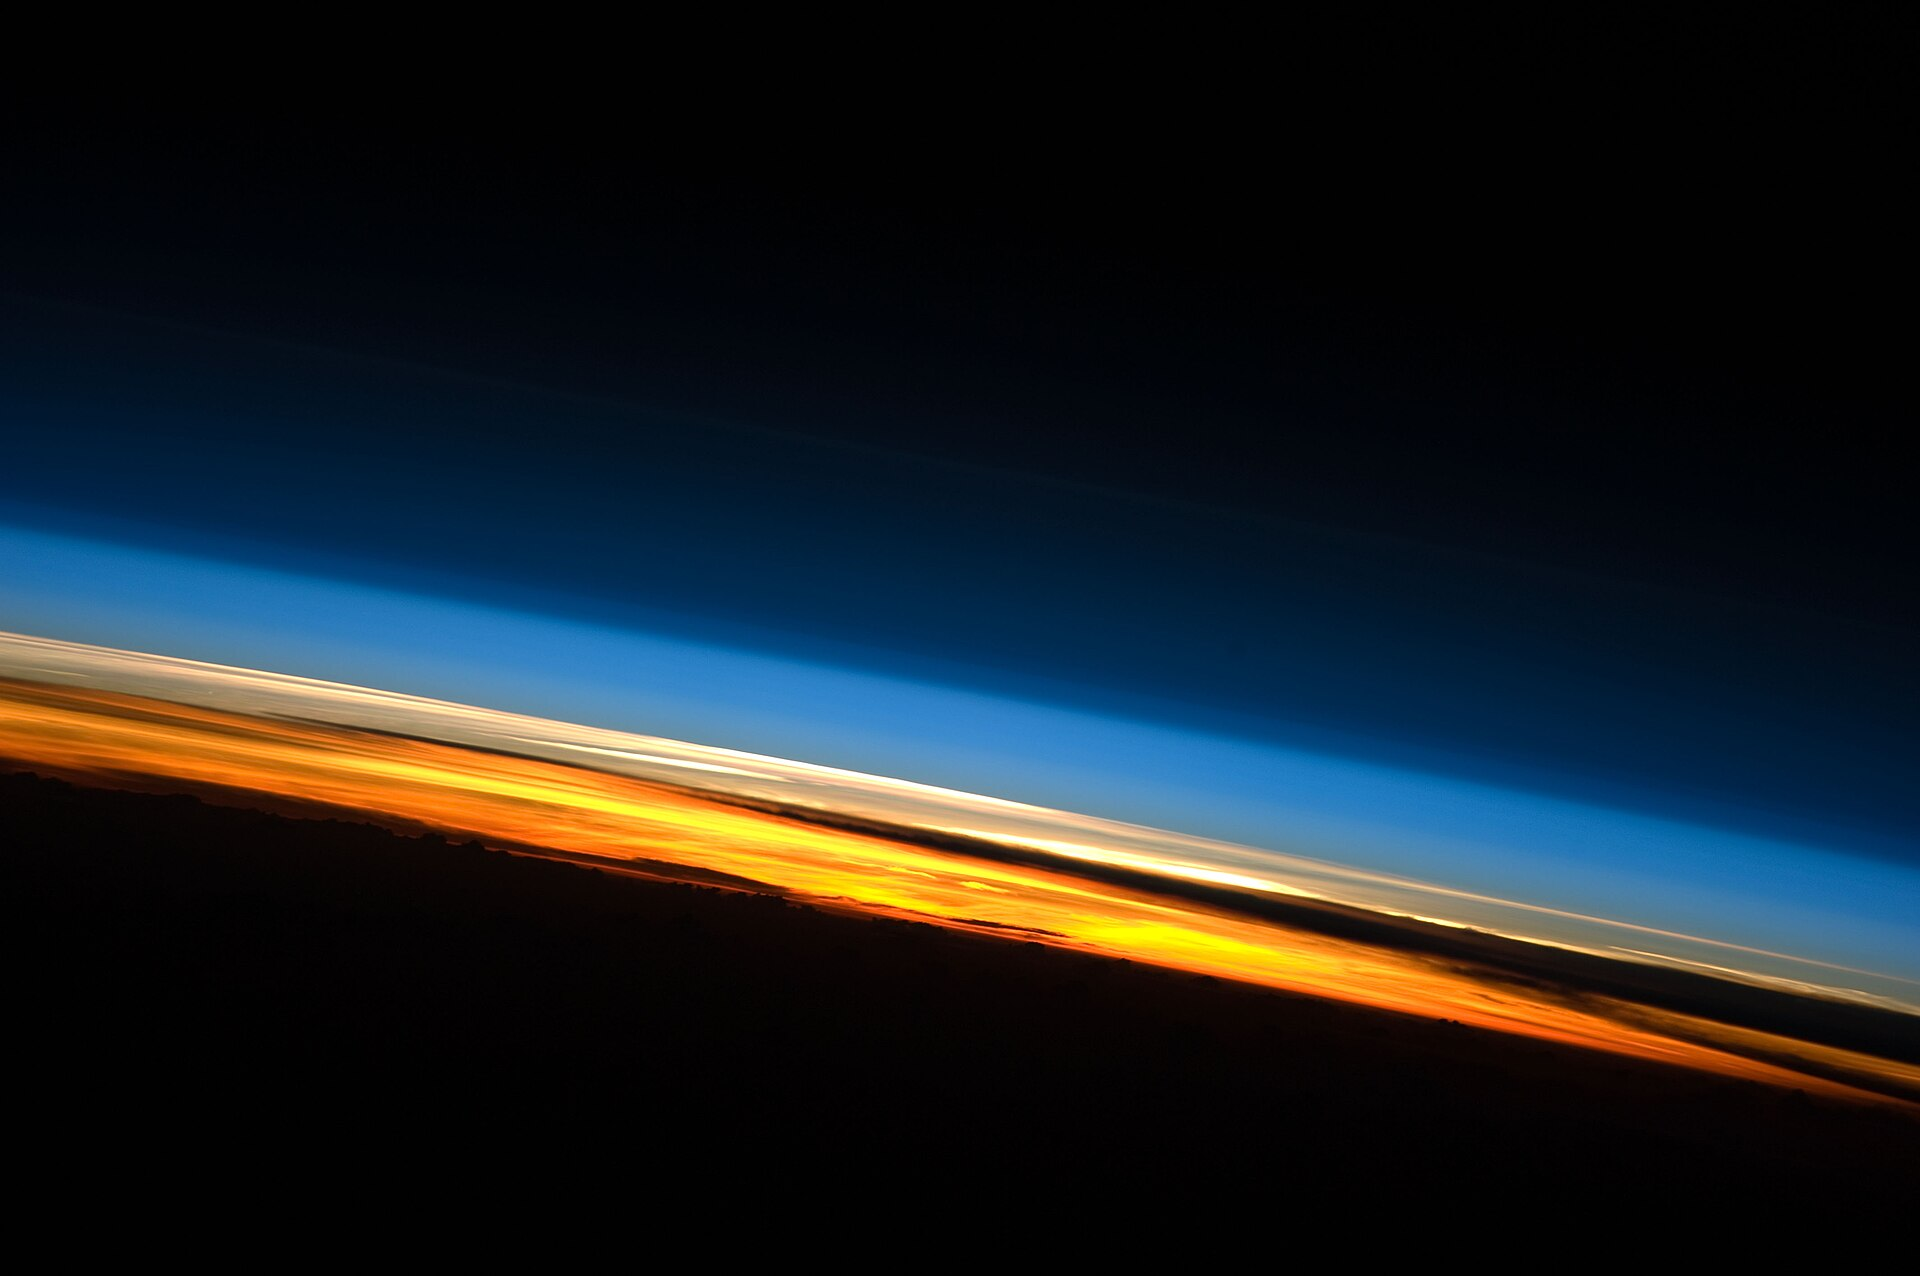
\includegraphics[width=0.78\linewidth]{images/book1/g8-iss-limb.jpg}

{\small Le bord de la Terre au coucher du Soleil, photographié depuis la
Station spatiale internationale au-dessus de l'\omterm{def:g2:water-on-earth:ocean}{océan} Indien, le 14~juin
2010. La bande orange et jaune est la couche la plus basse de
l'atmosphère, avec ses \omterm{def:g4:clouds-rain-snow:cloud}{nuages} sombres~; au-dessus viennent des couches
plus pâles, puis bleues, qui se fondent dans le noir de l'espace.
Photographie de la NASA, ISS Expedition~23 (domaine public, via
Wikimedia Commons).}
% ledger: commons:iss-sunset
\label{fig:g8:the-atmosphere:limb}
\end{omfigure}

L'atmosphère n'a pas de sommet net~: l'air devient de plus en plus rare
avec l'\omterm{def:g4:world-physical-map:altitude}{altitude}. Par convention, l'espace commence vers \qty{100}{km}.
Comparé au rayon de la Terre, \qty{6371}{km}, c'est très peu~: $100 \div
6371 \approx 0.016$, moins de 2~\% du rayon. Sur un \omterm{def:g3:continents-and-oceans:globe}{globe} de
\qty{30}{cm} de diamètre, toute l'atmosphère serait une pellicule
d'environ \qty{2}{mm} d'épaisseur.
% ledger: ucar:layers, earth:Rmean

\begin{omfigure}
\begin{tikzpicture}[font=\footnotesize]
  % 1 cm = 100 km: the Earth's surface is a circle of radius 63.71 cm
  \def\R{63.71}
  \useasboundingbox (-6.9,-1.6) rectangle (6.9,1.0);
  \fill[blue!8] (0,-\R) ++(85:\R+1) arc (85:95:\R+1) -- ($(0,-\R)+(95:\R)$) arc (95:85:\R) -- cycle;
  \fill[omLithAlluv!70] (0,-\R) ++(85:\R) arc (85:95:\R) -- ++(0,-0.6) -- ($(0,-\R)+(85:\R)+(0,-0.6)$) -- cycle;
  \draw[black, line width=0.6pt] (0,-\R) ++(85:\R) arc (85:95:\R);
  \foreach \h/\c in {0.1102/omThm, 0.4938/omMeth, 0.86/omDef} \draw[\c, line width=0.5pt] (0,-\R) ++(85:\R+\h) arc (85:95:\R+\h);
  \draw[black!60, dashed] (0,-\R) ++(85:\R+1) arc (85:95:\R+1);
  \node[anchor=west, omThm] at (5.65,-0.14) {\qty{11}{km}};
  \node[anchor=west, omMeth] at (5.65,0.25) {\qty{49}{km}};
  \node[anchor=west, omDef] at (5.65,0.62) {\qty{86}{km}};
  \node[anchor=east, black!70] at (-5.65,0.75) {\qty{100}{km}};
  \node[anchor=north] at (0,-0.15) {la surface de la Terre};
  \draw[|-|] (-5,-1.05) -- node[below] {\qty{1000}{km}} (5,-1.05);
\end{tikzpicture}

{\small Une tranche de la Terre et de son atmosphère dessinée à l'échelle
(\qty{1}{cm} pour \qty{100}{km}), jusqu'à \qty{100}{km}, la limite de
l'espace (en tirets). Les lignes de couleur sont les limites des couches
rencontrées plus loin dans ce chapitre~; la couche la plus basse, où se
produit toute la \omterm{def:g1:watching-the-weather:weather}{météo}, a à peine un millimètre d'épaisseur.}
% ledger: earth:Rmean, ucar:layers (limits: figdata/grade-8/standard_atmosphere.py main table)
\label{fig:g8:the-atmosphere:to-scale}
\end{omfigure}

\section{La pression baisse avec l'altitude}

L'air du bas de l'atmosphère porte le poids de tout l'air situé au-dessus.
Plus on monte, moins il reste d'air au-dessus de soi, et plus la pression
est faible. Dans le modèle standard de l'atmosphère qu'utilisent les
météorologues et les ingénieurs, la pression vaut \qty{1013}{hPa} au
\omterm{def:g4:world-physical-map:altitude}{niveau de la mer}, la moitié vers \qty{5.5}{km}, et le quart vers
\qty{10.3}{km}.
% ledger: ussa76:sea-level, ussa76:layers (figdata/grade-8/standard_atmosphere.py main table: half_km 5.48, quarter_km 10.29)

Puisque la pression mesure le poids de l'air situé au-dessus, le niveau de
la demi-pression est aussi l'\omterm{def:g4:world-physical-map:altitude}{altitude} au-dessous de laquelle se trouve la
moitié de tout l'air~: la moitié de l'atmosphère est tassée dans ses
\qty{5.5}{km} les plus bas. Au-dessous de \qty{11}{km} se trouve environ
78~\% de l'air, au-dessous de \qty{30}{km} environ 99~\%.
% ledger: (computed: figdata/grade-8/standard_atmosphere.py, share_below_11km 77.7, share_below_30km 98.82)

\begin{omfigure}
\begin{minipage}[t]{0.49\linewidth}\centering
\begin{tikzpicture}
\begin{axis}[width=6.6cm, height=7.6cm, xmin=0, xmax=1100, ymin=0, ymax=30,
  xlabel={pression (hPa)}, ylabel={altitude (km)},
  tick label style={font=\scriptsize}, label style={font=\small},
  xtick={0,250,500,750,1000}, ytick={0,5,10,15,20,25,30}]
  \addplot[dashed, black!60] table {figdata/out/grade-8-standard_atmosphere-guides.dat};
  \addplot[omDef, line width=1.1pt] table[x=p_hPa, y=z_km] {figdata/out/grade-8-standard_atmosphere-pressure.dat};
  \addplot[only marks, mark=*, mark size=1.8pt, omThm] table[x=p_hPa, y=z_km] {figdata/out/grade-8-standard_atmosphere-levels.dat};
  \node[anchor=south west, font=\scriptsize, text=black] at (axis cs:506.6,5.48) {moitié};
  \node[anchor=south west, font=\scriptsize, text=black] at (axis cs:253.3,10.29) {quart};
\end{axis}
\end{tikzpicture}

{\small La pression en fonction de l'\omterm{def:g4:world-physical-map:altitude}{altitude}. La pression vaut la moitié
de sa valeur au \omterm{def:g4:world-physical-map:altitude}{niveau de la mer} vers \qty{5.5}{km}, le quart vers
\qty{10.3}{km}.}
\end{minipage}\hfill
\begin{minipage}[t]{0.49\linewidth}\centering
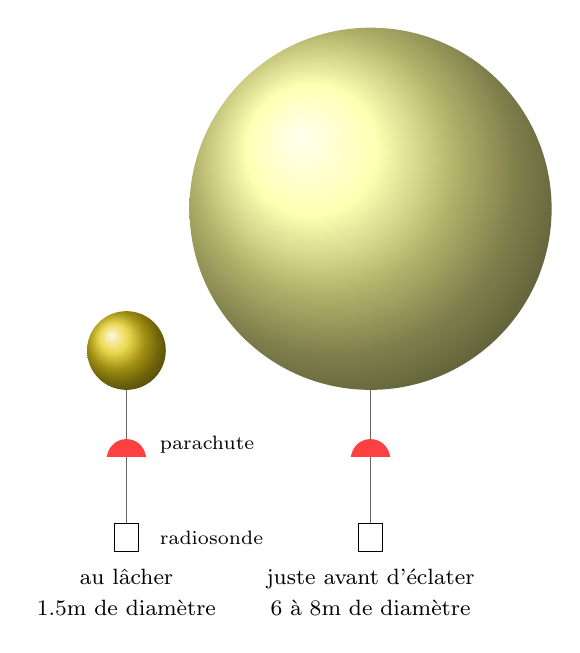
\begin{tikzpicture}[font=\footnotesize]
  % at launch: 1.5 m; at burst: about 7 m (drawn 1 cm for 1.5 m)
  \draw[black!60] (0,0.9) -- (0,2.6);
  \shade[ball color=yellow!60!brown] (0,3.1) circle (0.5);
  \fill[red!75] (-0.25,1.75) .. controls (-0.2,2.05) and (0.2,2.05) .. (0.25,1.75) -- cycle;
  \fill[white, draw=black] (-0.15,0.55) rectangle (0.15,0.9);
  \node[anchor=north] at (0,0.45) {au lâcher};
  \node[anchor=north] at (0,0.05) {\qty{1.5}{m} de diamètre};
  \begin{scope}[xshift=3.1cm]
    \draw[black!60] (0,0.9) -- (0,2.6);
    \shade[ball color=yellow!40!white] (0,4.9) circle (2.3);
    \fill[red!75] (-0.25,1.75) .. controls (-0.2,2.05) and (0.2,2.05) .. (0.25,1.75) -- cycle;
    \fill[white, draw=black] (-0.15,0.55) rectangle (0.15,0.9);
    \node[anchor=north] at (0,0.45) {juste avant d'éclater};
    \node[anchor=north] at (0,0.05) {6 à \qty{8}{m} de diamètre};
  \end{scope}
  \node[anchor=west, font=\scriptsize] at (0.3,1.9) {parachute};
  \node[anchor=west, font=\scriptsize] at (0.3,0.72) {radiosonde};
\end{tikzpicture}

{\small Le ballon gonfle en montant, parce que l'air qui l'entoure appuie
de moins en moins (ballons et parachutes à la même échelle, la ficelle
raccourcie).}
% ledger: nws:radiosonde
\end{minipage}
% ledger: ussa76:sea-level, ussa76:layers (figdata/grade-8/standard_atmosphere.py parts pressure, levels, guides)
\label{fig:g8:the-atmosphere:pressure}
\end{omfigure}

Plus haut, la pression continue de baisser, d'environ moitié encore tous
les quelques kilomètres~: elle devient vite minuscule. Les puissances de
dix sont la meilleure façon de l'écrire. À \qty{30}{km}, la pression vaut
environ \qty{12}{hPa}, à peu près $10^{-2}$ de sa valeur au \omterm{def:g4:world-physical-map:altitude}{niveau de la
mer} (un centième)~; à \qty{50}{km}, environ \qty{0.8}{hPa}, à peu près
$10^{-3}$~; à \qty{80}{km}, environ \qty{0.01}{hPa}, à peu près $10^{-5}$
de la pression au \omterm{def:g4:world-physical-map:altitude}{niveau de la mer}.
% ledger: ussa76:layers (figdata/grade-8/standard_atmosphere.py main table: p_30km 11.97, p_50km 0.798, p_80km 0.0105 hPa)

\begin{omfigure}
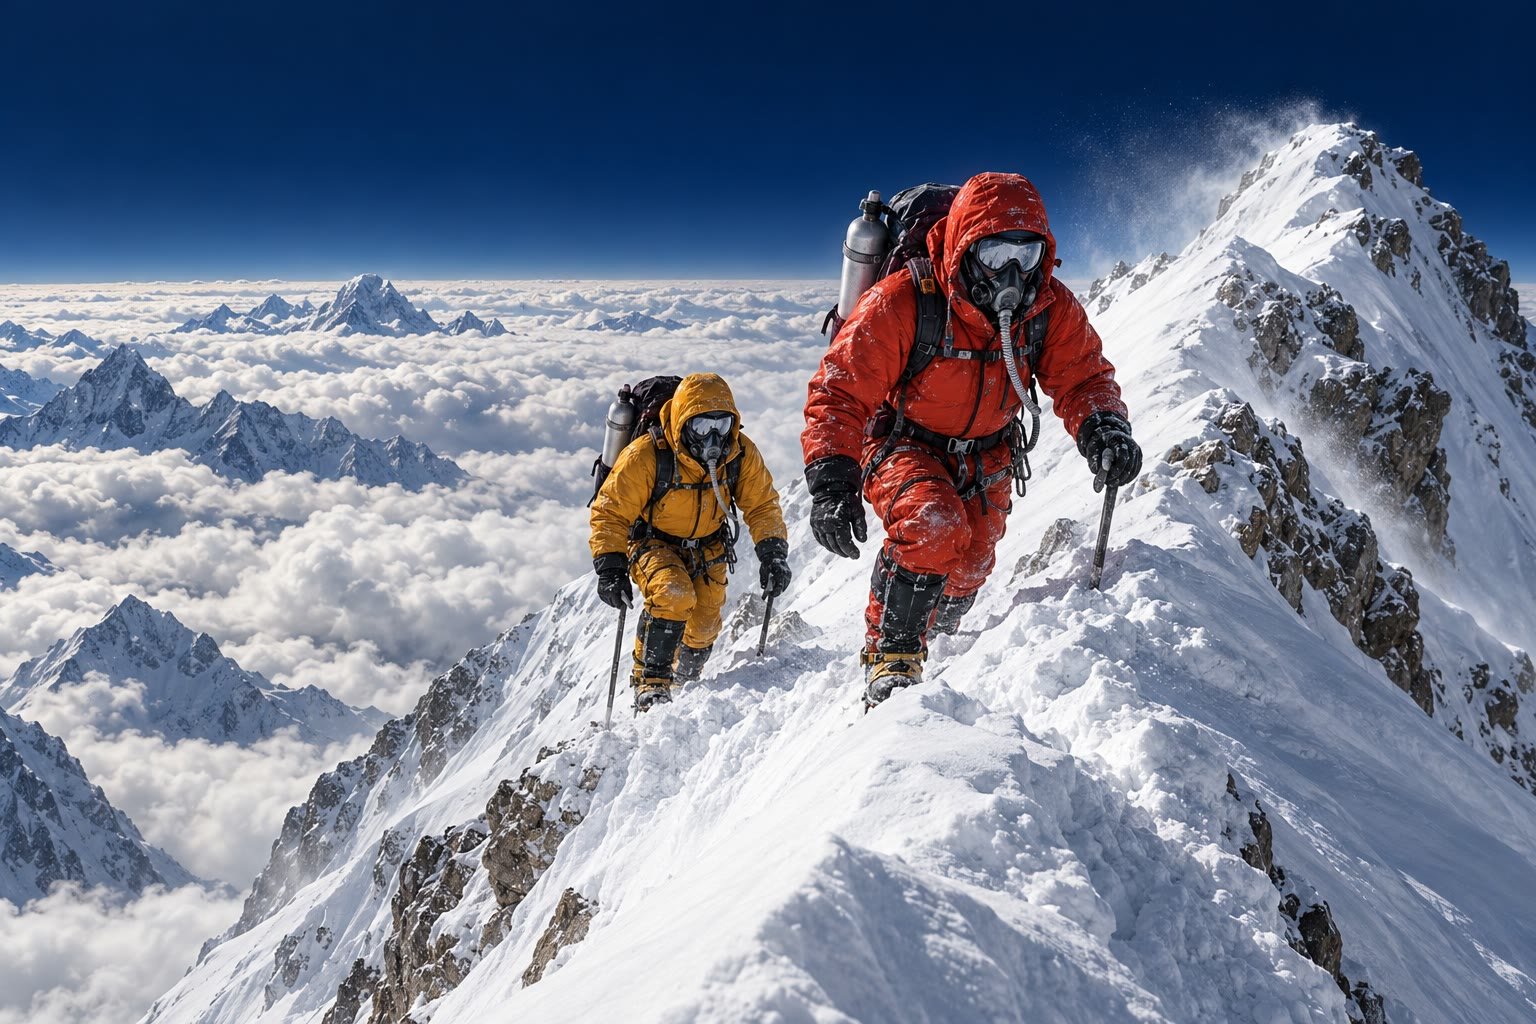
\includegraphics[width=0.5\linewidth]{images/book1/ai/g8-climbers.jpg}

{\small Des alpinistes sur une très haute \omterm{def:g1:landscapes-around-us:landform}{montagne} portent des bouteilles
d'oxygène. À \qty{9}{km}, la pression est inférieure au tiers de sa
valeur au \omterm{def:g4:world-physical-map:altitude}{niveau de la mer}~: l'air contient toujours 21~\% d'oxygène, mais
chaque inspiration en apporte bien moins (illustration générée par IA
d'une scène générique).}
% ledger: air:O2 (figdata/grade-8/standard_atmosphere.py: pressure at 9 km 308 hPa, 30 % of sea level)
\label{fig:g8:the-atmosphere:climbers}
\end{omfigure}

\section{La température et les couches}

Quiconque a gravi une \omterm{def:g1:landscapes-around-us:landform}{montagne} sait que l'air se refroidit avec
l'\omterm{def:g4:world-physical-map:altitude}{altitude}. Les radiosondes montrent que ce n'est vrai que dans la partie
la plus basse de l'atmosphère. Plus haut, la température cesse de baisser,
puis monte, puis baisse de nouveau, puis monte encore. Ces changements
partagent l'atmosphère en couches.
% ledger: ucar:layers, ussa76:layers

\begin{omfigure}
\begin{tikzpicture}
\begin{axis}[width=10cm, height=9cm, xmin=-100, xmax=30, ymin=0, ymax=100,
  xlabel={température ($^\circ$C)}, ylabel={altitude (km)},
  tick label style={font=\scriptsize}, label style={font=\small},
  xtick={-100,-80,-60,-40,-20,0,20}, ytick={0,10,20,30,40,50,60,70,80,90,100}, axis on top]
  \addplot[fill=omSea!55, draw=none] table {figdata/out/grade-8-standard_atmosphere-band-troposphere.dat};
  \addplot[fill=omMeth!12, draw=none] table {figdata/out/grade-8-standard_atmosphere-band-stratosphere.dat};
  \addplot[fill=omSea!35, draw=none] table {figdata/out/grade-8-standard_atmosphere-band-mesosphere.dat};
  \addplot[fill=omThm!10, draw=none] table {figdata/out/grade-8-standard_atmosphere-band-thermosphere.dat};
  \addplot[omThm, line width=1.2pt] table[x=T_C, y=z_km] {figdata/out/grade-8-standard_atmosphere-temp.dat};
  \node[anchor=west, font=\small\bfseries, text=black!75] at (axis cs:-97,5.51) {troposphère};
  \node[anchor=west, font=\small\bfseries, text=black!75] at (axis cs:-97,30.2) {stratosphère};
  \node[anchor=west, font=\small\bfseries, text=black!75] at (axis cs:-97,67.69) {mésosphère};
  \node[anchor=west, font=\small\bfseries, text=black!75] at (axis cs:-60,93) {thermosphère};
  \draw[black!50, dashed] (axis cs:-100,11.02) -- (axis cs:30,11.02);
  \draw[black!50, dashed] (axis cs:-100,49.38) -- (axis cs:30,49.38);
  \draw[black!50, dashed] (axis cs:-100,86) -- (axis cs:30,86);
  \node[anchor=south east, font=\scriptsize] at (axis cs:17,11.02) {tropopause};
  \node[anchor=south east, font=\scriptsize] at (axis cs:29,49.38) {stratopause};
  \node[anchor=south east, font=\scriptsize] at (axis cs:29,86) {mésopause};
  \fill[omMeth!45] (axis cs:19,16) rectangle (axis cs:23,48);
  \node[anchor=east, font=\scriptsize, align=right] at (axis cs:18,30) {couche\\d'ozone};
\end{axis}
\end{tikzpicture}

{\small La température de l'air en fonction de l'\omterm{def:g4:world-physical-map:altitude}{altitude}, du sol jusqu'à
\qty{100}{km}, dans l'atmosphère standard (une moyenne pour les \omterm{def:g6:latitude-longitude:latitude}{latitudes}
moyennes). Les quatre couches sont colorées~; la barre verte marque
l'\omterm{def:g4:world-physical-map:altitude}{altitude} de la \omterm{def:g8:the-atmosphere:ozone-layer}{couche d'ozone}.}
% ledger: ussa76:sea-level, ussa76:layers, ussa76:above-86, ucar:ozone (figdata/grade-8/standard_atmosphere.py parts temp, layers, band-*)
\label{fig:g8:the-atmosphere:temperature}
\end{omfigure}

\begin{definition}[Les couches de l'atmosphère]\label{def:g8:the-atmosphere:layers}
Du sol vers le haut, l'atmosphère est partagée en quatre couches selon la
façon dont sa température varie avec l'\omterm{def:g4:world-physical-map:altitude}{altitude}~:
\begin{itemize}
  \item la \emph{troposphère}\index{troposphere@troposphère}, où la
        température baisse avec l'\omterm{def:g4:world-physical-map:altitude}{altitude} et où se produit presque toute
        la \omterm{def:g1:watching-the-weather:weather}{météo}~; son sommet est la \emph{tropopause}\index{tropopause}~;
  \item la \emph{stratosphère}\index{stratosphere@stratosphère}, où la
        température monte avec l'\omterm{def:g4:world-physical-map:altitude}{altitude}, jusque vers \qty{50}{km}~;
  \item la \emph{mésosphère}\index{mesosphere@mésosphère}, où la
        température baisse de nouveau, jusque vers \qty{85}{km}~;
  \item la \emph{thermosphère}\index{thermosphere@thermosphère}, où l'air,
        très rare, devient de plus en plus chaud avec l'\omterm{def:g4:world-physical-map:altitude}{altitude}.
\end{itemize}
\end{definition}
% ledger: ucar:layers, ussa76:layers

La \omterm{def:g8:the-atmosphere:layers}{troposphère} contient environ 99~\% de la vapeur d'eau de l'atmosphère~:
presque tous les \omterm{def:g4:clouds-rain-snow:cloud}{nuages}, la \omterm{def:g4:clouds-rain-snow:precipitation}{pluie} et la \omterm{def:g4:clouds-rain-snow:precipitation}{neige} s'y forment. Son air est
brassé en permanence. Le sommet de la \omterm{def:g8:the-atmosphere:layers}{troposphère} n'est pas à la même
\omterm{def:g4:world-physical-map:altitude}{altitude} partout~: la \omterm{def:g8:the-atmosphere:layers}{tropopause} est la plus haute au-dessus de l'\omterm{def:g3:continents-and-oceans:equator}{équateur},
où elle peut atteindre \qty{20}{km}, et la plus basse au-dessus des \omterm{def:g3:continents-and-oceans:poles}{pôles},
où elle peut descendre à \qty{7}{km} en hiver. Elle est aussi plus haute
en été qu'en hiver. Dans l'atmosphère standard, une moyenne pour les
\omterm{def:g6:latitude-longitude:latitude}{latitudes} moyennes, elle se trouve à \qty{11}{km}.
% ledger: ucar:layers, ucar:tropopause, ussa76:layers

\begin{definition}[Gradient thermique vertical]\label{def:g8:the-atmosphere:lapse-rate}
Le \emph{gradient thermique vertical}\index{gradient thermique vertical}
est la vitesse à laquelle la température de l'air baisse avec l'\omterm{def:g4:world-physical-map:altitude}{altitude}
dans la \omterm{def:g8:the-atmosphere:layers}{troposphère}, en degrés Celsius par kilomètre. Il change d'un jour à
l'autre et d'un lieu à l'autre~; l'atmosphère standard utilise une moyenne
de \qty{6.5}{\degreeCelsius} par kilomètre.
\end{definition}
% ledger: ussa76:layers

\begin{method}[Lire un profil de température]\label{met:g8:the-atmosphere:profile}
\begin{enumerate}
  \item Repère l'\omterm{def:g4:world-physical-map:altitude}{altitude} sur l'axe vertical et va horizontalement jusqu'à
        la courbe~; lis la température au-dessous.
  \item Là où la courbe penche vers la gauche en montant, l'air se
        refroidit avec l'\omterm{def:g4:world-physical-map:altitude}{altitude}~; là où elle penche vers la droite, l'air
        se réchauffe avec l'\omterm{def:g4:world-physical-map:altitude}{altitude}~; là où elle est verticale, la
        température ne change pas.
  \item Les limites entre les couches sont là où la courbe tourne.
\end{enumerate}
\end{method}

\begin{example}[Un avion de ligne à son altitude de croisière]\label{ex:g8:the-atmosphere:airliner}
Un avion de ligne vole à \qty{11}{km}, près de la \omterm{def:g8:the-atmosphere:layers}{tropopause}. Sur le
profil, la température y est d'environ \qty{-56}{\degreeCelsius}. Avec le
gradient~: à partir de \qty{15}{\degreeCelsius} au \omterm{def:g4:world-physical-map:altitude}{niveau de la mer},
l'air se refroidit de $6.5 \times 11 = 71.5$ degrés, ce qui donne $15 - 71.5 =
\qty{-56.5}{\degreeCelsius}$. Sur la courbe de pression, la pression vaut
environ \qty{227}{hPa}, moins du quart de la pression au sol~: la cabine
doit être pressurisée.
% ledger: ussa76:sea-level, ussa76:layers (figdata/grade-8/standard_atmosphere.py: T at 11 km -56.4 degC, p 227 hPa)
\end{example}

Au-dessus de la \omterm{def:g8:the-atmosphere:layers}{tropopause}, dans la \omterm{def:g8:the-atmosphere:layers}{stratosphère}, les avions de ligne
trouvent un vol plus calme~: l'air y devient plus chaud avec l'\omterm{def:g4:world-physical-map:altitude}{altitude},
il n'est donc pas brassé par le bas. Dans la \omterm{def:g8:the-atmosphere:layers}{mésosphère}, la plupart des
météores se consument, et à son sommet, vers \qty{86}{km}, se trouve l'air
le plus froid de toute l'atmosphère, environ \qty{-86}{\degreeCelsius}.
Dans la \omterm{def:g8:the-atmosphere:layers}{thermosphère}, les rayons X et la lumière ultraviolette du Soleil
chauffent l'air très rare à des centaines, parfois des milliers de
degrés~; pourtant, il y a si peu d'air qu'il ne paraîtrait pas chaud. De
nombreux satellites tournent autour de la Terre à cette \omterm{def:g4:world-physical-map:altitude}{altitude}.
% ledger: ucar:layers, ussa76:above-86

\section{La couche d'ozone}

La \omterm{def:g8:the-atmosphere:layers}{stratosphère} devient plus chaude avec l'\omterm{def:g4:world-physical-map:altitude}{altitude} parce qu'elle absorbe
une partie de la lumière du Soleil. Le gaz qui en absorbe la plus grande
part est l'ozone, une forme de l'oxygène (sa chimie est dans les livres de
chimie).

\begin{definition}[Couche d'ozone]\label{def:g8:the-atmosphere:ozone-layer}
La \emph{couche d'ozone}\index{couche d'ozone} est la partie de la
\omterm{def:g8:the-atmosphere:layers}{stratosphère}, entre environ \qty{16}{km} et \qty{48}{km}, où se trouve
environ 90~\% de l'ozone de l'atmosphère. Elle absorbe la plus grande
partie de la lumière ultraviolette nocive du Soleil.
\end{definition}
% ledger: ucar:ozone

Même dans la \omterm{def:g8:the-atmosphere:ozone-layer}{couche d'ozone}, l'ozone est rare~: seulement 1 à
10~molécules sur un million. Pourtant, avec l'oxygène, il arrête entre
95~\% et 99.9~\% de la lumière ultraviolette qui atteint la Terre, y
compris les sortes les plus nocives. L'énergie qu'il absorbe est changée
en chaleur~: c'est pourquoi la température monte à travers la
\omterm{def:g8:the-atmosphere:layers}{stratosphère}. Sans la \omterm{def:g8:the-atmosphere:ozone-layer}{couche d'ozone}, la lumière ultraviolette qui
atteindrait le sol nuirait aux êtres vivants.
% ledger: ucar:ozone

\begin{inthefield}[Suivre les ballons-sondes]
Les services \omterm{def:g1:watching-the-weather:weather}{météorologiques} publient les mesures de leurs radiosondes,
souvent sous la forme d'un graphique de la température en fonction de
l'\omterm{def:g4:world-physical-map:altitude}{altitude} pour chaque lâcher. Avec un adulte, cherche les sondages de la
station la plus proche de chez toi, faits à 0~h ou à 12~h~UTC. Trouve
l'\omterm{def:g4:world-physical-map:altitude}{altitude} où la température cesse de baisser~: c'est la \omterm{def:g8:the-atmosphere:layers}{tropopause} ce
jour-là. Compare un sondage d'hiver avec un sondage d'été.
\end{inthefield}
% ledger: nws:radiosonde, ucar:tropopause

\section{Exercices}

\begin{exercise}[$\star$]\label{exo:g8:the-atmosphere:1}
Associe chaque couche à sa description~: \omterm{def:g8:the-atmosphere:layers}{troposphère}~; \omterm{def:g8:the-atmosphere:layers}{stratosphère}~;
\omterm{def:g8:the-atmosphere:layers}{mésosphère}~; \omterm{def:g8:the-atmosphere:layers}{thermosphère}. (a) La température monte avec l'\omterm{def:g4:world-physical-map:altitude}{altitude} et la
\omterm{def:g8:the-atmosphere:ozone-layer}{couche d'ozone} s'y trouve. (b) Presque toute la \omterm{def:g1:watching-the-weather:weather}{météo} s'y produit. (c)
L'air le plus froid de l'atmosphère se trouve à son sommet. (d) L'air,
très rare, y est chauffé à des centaines de degrés~; de nombreux
satellites y tournent.
\end{exercise}

\begin{exercise}[$\star$]\label{exo:g8:the-atmosphere:2}
Utilise le profil de température de l'atmosphère standard. (a) Quelle est
la température au \omterm{def:g4:world-physical-map:altitude}{niveau de la mer}~? (b) À \qty{11}{km}~? (c) À
\qty{50}{km}~? (d) À \qty{86}{km}~? (e) Entre quelles \omterm{def:g4:world-physical-map:altitude}{altitudes} la
température ne change-t-elle pas~?
\end{exercise}

\begin{exercise}[$\star$]\label{exo:g8:the-atmosphere:3}
Vrai ou faux~? Corrige les phrases fausses. (a) La température de l'air
baisse toujours avec l'\omterm{def:g4:world-physical-map:altitude}{altitude}. (b) La moitié de tout l'air se trouve
au-dessous de \qty{5.5}{km} environ. (c) La \omterm{def:g8:the-atmosphere:ozone-layer}{couche d'ozone} se trouve dans
la \omterm{def:g8:the-atmosphere:layers}{troposphère}. (d) La \omterm{def:g8:the-atmosphere:layers}{tropopause} est plus haute au-dessus de l'\omterm{def:g3:continents-and-oceans:equator}{équateur}
qu'au-dessus des \omterm{def:g3:continents-and-oceans:poles}{pôles}.
\end{exercise}

\begin{exercise}[$\star$]\label{exo:g8:the-atmosphere:4}
Dans quelle couche se trouve chacun de ces objets~? (a) Un \omterm{def:g4:clouds-rain-snow:cloud}{nuage} de \omterm{def:g4:clouds-rain-snow:precipitation}{pluie}.
(b) Un avion de ligne à \qty{12}{km}. (c) Un ballon-sonde juste avant
d'éclater, à \qty{32}{km}. (d) Un météore qui se consume à \qty{75}{km}.
\end{exercise}

\begin{exercise}[$\star\star$]\label{exo:g8:the-atmosphere:5}
Un jour d'été, il fait \qty{20}{\degreeCelsius} au \omterm{def:g4:world-physical-map:altitude}{niveau de la mer}.
Suppose que l'air se refroidisse de \qty{6.5}{\degreeCelsius} par
kilomètre. (a) Quelle est la température à \qty{2}{km}~? (b) À
\qty{3}{km}~? (c) Vers quelle \omterm{def:g4:world-physical-map:altitude}{altitude} l'air atteint-il
\qty{0}{\degreeCelsius}~? Arrondis au dixième.
\end{exercise}

\begin{exercise}[$\star\star$]\label{exo:g8:the-atmosphere:6}
Un refuge de \omterm{def:g1:landscapes-around-us:landform}{montagne} se trouve à \qty{3000}{m}. Un randonneur part d'un
village situé à \qty{500}{m}, où il fait \qty{18}{\degreeCelsius}. Avec un
gradient de \qty{6.5}{\degreeCelsius} par kilomètre~: (a) De combien de
kilomètres le randonneur monte-t-il~? (b) De combien de degrés l'air se
refroidit-il~? (c) Quelle température le randonneur peut-il attendre au
refuge~?
\end{exercise}

\begin{exercise}[$\star\star$]\label{exo:g8:the-atmosphere:7}
Suppose que la pression soit divisée par deux tous les \qty{5.5}{km}, à
partir de \qty{1000}{hPa} au \omterm{def:g4:world-physical-map:altitude}{niveau de la mer}. (a) Quelle est la pression
à \qty{5.5}{km}~? À \qty{11}{km}~? À \qty{16.5}{km}~? (b) L'atmosphère
standard donne environ \qty{506}{hPa}, \qty{227}{hPa} et \qty{96}{hPa} à
ces trois \omterm{def:g4:world-physical-map:altitude}{altitudes} (pour \qty{1013}{hPa} au \omterm{def:g4:world-physical-map:altitude}{niveau de la mer}). La règle
de la division par deux est-elle bonne près du sol~? Plus haut~?
\end{exercise}

\begin{exercise}[$\star\star$]\label{exo:g8:the-atmosphere:8}
Au \omterm{def:g4:world-physical-map:altitude}{niveau de la mer}, la pression vaut environ \qty{1000}{hPa}, soit
$10^3$~hPa. (a) À \qty{30}{km}, elle vaut environ \qty{10}{hPa}. Écris-la
sous forme de puissance de dix, et dis combien de fois elle est plus
petite qu'au \omterm{def:g4:world-physical-map:altitude}{niveau de la mer}. (b) À \qty{80}{km}, elle vaut environ
\qty{0.01}{hPa}. Écris-la sous forme de puissance de dix. (c) Combien de
fois est-elle plus petite qu'au \omterm{def:g4:world-physical-map:altitude}{niveau de la mer}~?
\end{exercise}

\begin{exercise}[$\star\star$]\label{exo:g8:the-atmosphere:9}
Un ballon-sonde mesure \qty{1.5}{m} de diamètre au lâcher et \qty{6}{m}
quand il éclate. (a) Combien de fois est-il plus large quand il éclate~?
(b) Explique pourquoi il gonfle en montant. (c) Pourquoi les services
\omterm{def:g1:watching-the-weather:weather}{météorologiques} accrochent-ils un parachute au-dessous~?
\end{exercise}

\begin{exercise}[$\star\star$]\label{exo:g8:the-atmosphere:10}
La \omterm{def:g8:the-atmosphere:layers}{tropopause} peut atteindre \qty{20}{km} au-dessus de l'\omterm{def:g3:continents-and-oceans:equator}{équateur} et
descendre à \qty{7}{km} au-dessus des \omterm{def:g3:continents-and-oceans:poles}{pôles} en hiver. (a) Dans ce cas,
combien de fois la \omterm{def:g8:the-atmosphere:layers}{troposphère} est-elle plus épaisse au-dessus de
l'\omterm{def:g3:continents-and-oceans:equator}{équateur}~? Arrondis au dixième. (b) Sur le profil standard, la
\omterm{def:g8:the-atmosphere:layers}{tropopause} est à \qty{11}{km}. L'atmosphère standard est-elle plus proche
de celle de l'\omterm{def:g3:continents-and-oceans:equator}{équateur} ou de celle des \omterm{def:g3:continents-and-oceans:poles}{pôles}~? (c) Un pilote vole d'une
région polaire jusqu'à l'\omterm{def:g3:continents-and-oceans:equator}{équateur} à une \omterm{def:g4:world-physical-map:altitude}{altitude} constante de
\qty{10}{km}. L'avion est-il dans la \omterm{def:g8:the-atmosphere:layers}{troposphère} ou dans la \omterm{def:g8:the-atmosphere:layers}{stratosphère}
au départ (en hiver)~? À l'arrivée~?
\end{exercise}

\begin{exercise}[$\star\star\star$]\label{exo:g8:the-atmosphere:11}
La part de tout l'air qui se trouve au-dessous d'une \omterm{def:g4:world-physical-map:altitude}{altitude} est $1 - p \div
p_0$, où $p$ est la pression à cette \omterm{def:g4:world-physical-map:altitude}{altitude} et $p_0 =
\qty{1013}{hPa}$ la pression au \omterm{def:g4:world-physical-map:altitude}{niveau de la mer}. (a) À \qty{5.5}{km}, $p
\approx \qty{506}{hPa}$~: quelle part de l'air se trouve au-dessous~? (b) À
\qty{11}{km}, $p \approx \qty{227}{hPa}$. (c) À \qty{30}{km}, $p \approx
\qty{12}{hPa}$. Donne les réponses en pourcentage, arrondies à l'unité.
(d) Quelle part de l'air se trouve au-dessus de \qty{30}{km}~?
\end{exercise}

\begin{exercise}[$\star\star\star$]\label{exo:g8:the-atmosphere:12}
Un \omterm{def:g3:continents-and-oceans:globe}{globe} scolaire mesure \qty{30}{cm} de diamètre~: son rayon,
\qty{15}{cm}, représente donc le rayon de la Terre, \qty{6371}{km}. (a)
Combien de kilomètres \qty{1}{cm} du \omterm{def:g3:continents-and-oceans:globe}{globe} représente-t-il~? Arrondis au
kilomètre. (b) Quelle serait, en millimètres, l'épaisseur de l'atmosphère
jusqu'à \qty{100}{km} sur ce \omterm{def:g3:continents-and-oceans:globe}{globe}~? (c) Et celle de la \omterm{def:g8:the-atmosphere:layers}{troposphère},
épaisse de \qty{11}{km}~? (d) Une feuille de papier a une épaisseur
d'environ \qty{0.1}{mm}. Combien de feuilles faudrait-il pour faire la
\omterm{def:g8:the-atmosphere:layers}{troposphère} du \omterm{def:g3:continents-and-oceans:globe}{globe}~?
\end{exercise}

\section{Problème~: Suivre un ballon-sonde}

\begin{problem}[{Problème du week-end --- un ballon-sonde monte à travers
l'atmosphère~; ses températures montrent les couches, et ses pressions
montrent où il ne reste que le quart de la pression au niveau de la mer}]
\label{pb:g8:the-atmosphere:1}
% ledger: nws:radiosonde; the table is the standard atmosphere, figdata/grade-8/standard_atmosphere.py part sonde
Une radiosonde est lâchée depuis une station située au \omterm{def:g4:world-physical-map:altitude}{niveau de la mer}.
Son ballon monte à environ \qty{300}{m} par minute. Le tableau donne la
pression et la température qu'elle mesure (les valeurs de l'atmosphère
standard, arrondies).

\begin{center}\small
\begin{tabular}{|l|*{8}{c|}}
\hline
\omterm{def:g4:world-physical-map:altitude}{altitude} (km) & 0 & 2 & 4 & 6 & 8 & 10 & 12 & 14 \\
\hline
pression (hPa) & 1013 & 795 & 617 & 472 & 357 & 265 & 194 & 142 \\
\hline
température ($^\circ$C) & 15 & 2 & $-11$ & $-24$ & $-37$ & $-50$ & $-56$ & $-56$ \\
\hline
\hline
\omterm{def:g4:world-physical-map:altitude}{altitude} (km) & 16 & 18 & 20 & 22 & 24 & 26 & 28 & 30 \\
\hline
pression (hPa) & 104 & 76 & 55 & 40 & 30 & 22 & 16 & 12 \\
\hline
température ($^\circ$C) & $-56$ & $-56$ & $-56$ & $-55$ & $-53$ & $-51$ & $-49$ & $-47$ \\
\hline
\end{tabular}
\end{center}

\noindent\textbf{Partie I --- La montée.}\par\nopagebreak
\begin{enumerate}[beginpenalty=10000]
  \item De combien de mètres le ballon monte-t-il en 10~minutes~?
  \item Combien de temps lui faut-il pour atteindre \qty{6}{km}~? Et
        \qty{30}{km}~?
  \item Le ballon éclate à \qty{30}{km}. Combien de temps le vol a-t-il
        duré, en heures et en minutes~?
  \item Nomme la couche où se trouve le ballon à \qty{8}{km}, et celle où
        il se trouve quand il éclate.
\end{enumerate}

\noindent\textbf{Partie II --- La température.}\par\nopagebreak
\begin{enumerate}[resume, beginpenalty=10000]
  \item De combien de degrés la température baisse-t-elle entre le sol et
        \qty{10}{km}~?
  \item Quel est le gradient, en degrés par kilomètre, dans cette partie
        de la montée~?
  \item Entre quelles \omterm{def:g4:world-physical-map:altitude}{altitudes} la température reste-t-elle la même~? Où
        est la \omterm{def:g8:the-atmosphere:layers}{tropopause}~?
  \item Que devient la température au-dessus de \qty{20}{km}~? Quel gaz
        l'explique~?
\end{enumerate}

\noindent\textbf{Partie III --- La pression.}\par\nopagebreak
\begin{enumerate}[resume, beginpenalty=10000]
  \item Quelle est la moitié de la pression au \omterm{def:g4:world-physical-map:altitude}{niveau de la mer}~? Entre
        quelles \omterm{def:g4:world-physical-map:altitude}{altitudes} est-elle atteinte~?
  \item Quel est le quart de la pression au \omterm{def:g4:world-physical-map:altitude}{niveau de la mer}~? Arrondis à
        l'hectopascal.
  \item Entre quelles deux \omterm{def:g4:world-physical-map:altitude}{altitudes} du tableau ce quart est-il atteint~?
  \item La pression baisse de \qty{71}{hPa} entre \qty{10}{km} et
        \qty{12}{km}. En supposant qu'elle baisse régulièrement, vers quelle
        \omterm{def:g4:world-physical-map:altitude}{altitude} la pression vaut-elle le quart de sa valeur au \omterm{def:g4:world-physical-map:altitude}{niveau de la
        mer}~? Arrondis au dixième.
\end{enumerate}
\end{problem}
